%%%%%%%%%%%%%%%%%%%%%%%%%%%%%%%%%%%%%%%%%
% Kieker Monitoring Component
%
% $Date$
% $Rev$:
% $Author$


\chapter{\KiekerMonitoringPart{} Component}\label{chap:componentsMonitoring}

\NOTIFYBOX{The Java sources of this chapter, as well as a pre-compiled binary, %
can be found in the %
\file{\customComponentsBookstoreApplicationDirDistro{}/} directory of the %
binary release.}

\section{Monitoring Controller}\label{sec:componentsMonitoring:monitoringController}

The \class{MonitoringController} constructs and controls a \KiekerMonitoringPart{} %
instance. As depicted by the class diagram in Figure~\ref{fig:monitoringController:classdiagram}, it provides methods for\\

\enlargethispage{1cm}

\begin{figure}\centering % [H]
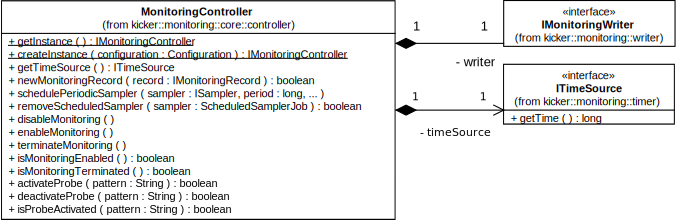
\includegraphics[scale=0.7]{images/kieker_monitoringControlleruserguide-simplified}
\caption{Class diagram of the \class{MonitoringController} (including selected methods)}
\label{fig:monitoringController:classdiagram}
\end{figure}

\begin{compactitem}
 \item Creating \class{IMonitoringController} instances (Section~\ref{sec:componentsMonitoring:monitoringController:factory}),
 \item Logging monitoring records with the configured monitoring writer (Section~\ref{sec:componentsMonitoring:monitoringController:logging}),
 \item Retrieving the current time via the configured time source (Section~\ref{sec:componentsMonitoring:monitoringController:getTime}),
 \item Scheduling and removing period samplers (Section~\ref{sec:componentsMonitoring:monitoringController:periodicSamplers}), and
 \item Controlling the monitoring state (Section~\ref{sec:componentsMonitoring:monitoringController:controState}).
\end{compactitem}

\subsection{Creating \class{MonitoringController} Instances}\label{sec:componentsMonitoring:monitoringController:factory}

The \class{MonitoringController} provides two different static methods for retrieving instances of %
\class{IMonitoringController}:\\

\begin{compactenum}
 \item The method \method{MonitoringController.getInstance()} returns a singleton instance. %
As described in Section~\ref{sec:monitoring:configuration}, the configuration is read from %
a properties file that has been passed to the JVM, is located in the classpath, or %
conforms to the default configuration (Appendix~\ref{sec:appdx:monitoringproperties}). %
 \item The method \method{MonitoringController.createInstance(Configuration config)} can be utilized to create %
an instance that is configured according to the passed \class{Configuration} object, %
as described in Section~\ref{sec:monitoring:configuration}.
\end{compactenum}

\subsection{Logging Monitoring Records}\label{sec:componentsMonitoring:monitoringController:logging}

Monitoring records are sent to the configured monitoring writers by passing %
these records, in form of \class{IMonitoringRecord} objects, to the %
\class{MonitoringController}'s \method{newMonitoringRecord} method.  %
Note, that this is not the case if monitoring is disabled or terminated (Section~\ref{sec:componentsMonitoring:monitoringController:controState}).

\subsection{Retrieving the Current Time and Using Custom Time Sources}\label{sec:componentsMonitoring:monitoringController:getTime}

The current time is maintained by a so-called time source. The \class{MonitoringController}'s method %
\method{getTimeSource} returns an \class{ITimeSource} whose method %
\method{getTime} returns a timestamp in nanoseconds. \Kieker{}'s default %
time source, \class{SystemNanoTimer}, returns the current system %
time as the number of nanoseconds elapsed since 1 Jan 1970 00:00~UTC. %
The easiest way to use a custom time source is to extend the \class{AbstractTimeSource} and %
to implement the method \method{getTime()}. Custom time sources make sense, for example, %
in simulations where not the current system time but the current simulation time is %
relevant. The configuration needs to be adjusted to use a custom time source class. %

\subsection{Scheduling and Removing Periodic Samplers}\label{sec:componentsMonitoring:monitoringController:periodicSamplers}

For certain applications, it is required to monitor runtime data periodically, %
e.g., the utilization of system resources such as CPUs. %
For this purpose, \Kieker{} supports special monitoring probes, called samplers. %
Samplers must implement the interface \class{ISampler} which includes a %
single method \method{sample(IMonitoringController monitoringController)}. %
This method is called in periodic time steps, %
as specified by the \class{MonitoringController}'s registration function %
\method{schedulePeriodicSampler}. Periodic samplers can be stopped by %
calling the \class{MonitoringController}'s method \method{removeScheduledSampler}.

Listing~\ref{listing:sigarSamplerMethod} shows the \method{sample} method %
of the \class{MemSwapUsageSampler} which can be used to monitor memory %
and swap usage employing the Sigar library~\cite{HypericSigarWebsite}. %
Likewise to other monitoring probes described in this user guide (see for %
example Sections~\ref{sec:monitoring:probe} and \ref{sec:example:monitoring}),
it collects the data of interest (lines~53--54), creates a monitoring record~%
(lines~55--58), and passes this monitoring record to the monitoring controller~%
(line~59). %
The available Sigar-based samplers for monitoring system-level monitoring %
data, such as CPU and memory usage, are discussed in Appendix~\ref{appendix:SigarBasedSamplers}. %

\pagebreak

\setJavaCodeListing
\lstinputlisting[firstline=47, lastline=60, firstnumber=47, caption=Method \method{sample} from MemSwapUsageSampler.java, label=listing:sigarSamplerMethod]{\kiekerSrcDir/monitoring/kieker/monitoring/probe/sigar/samplers/MemSwapUsageSampler.java}

\subsection{Controlling the Monitoring State}\label{sec:componentsMonitoring:monitoringController:controState}

The \class{MonitoringController} provides methods to temporarily enable or disable monitoring %
(\method{enableMonitoring}/\method{disableMonitoring}), as well as to terminate monitoring %
permanently (\method{terminateMonitoring}). %
The current state can be requested by calling the methods \method{isMonitoringEnabled} %
and \method{isMonitoringTerminated}. If monitoring is not enabled (i.e., disabled %
or terminated), no monitoring records retrieved via the method \method{newMonitoringRecord} %
are passed to the monitoring writer. Also, probes should be passive or return immediately %
with respect to the return value of the method \method{isMonitoringEnabled}. %
Note, that once the \class{MonitoringController} is terminated, it cannot be enabled %
later on.

\subsection{JMX MBean Access to \class{MonitoringController}}

\begin{figure}\centering
\subfigure[Attributes]{%
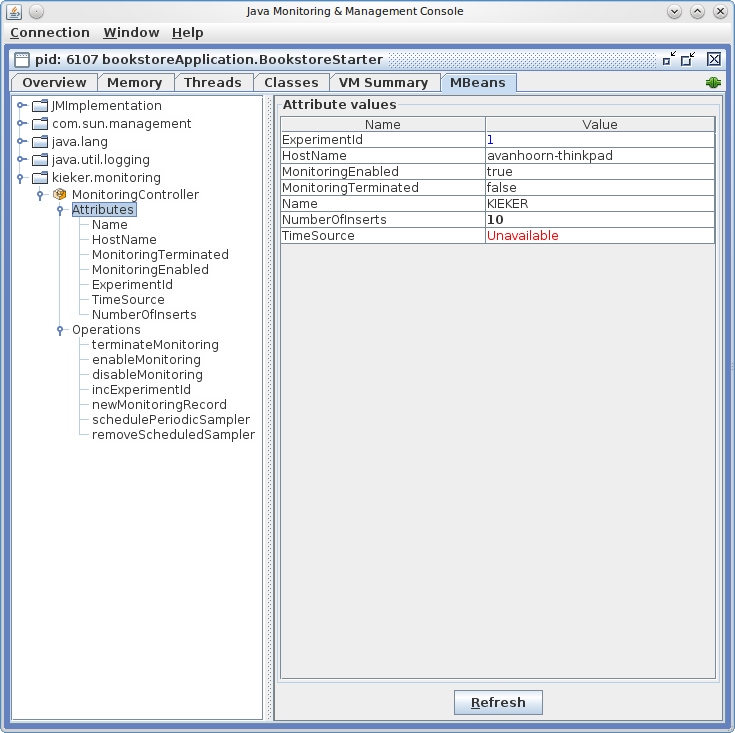
\includegraphics[width=0.485\textwidth]{images/jmxbean-monitoringcontroller-attributes.png}
}
\subfigure[Operations]{%
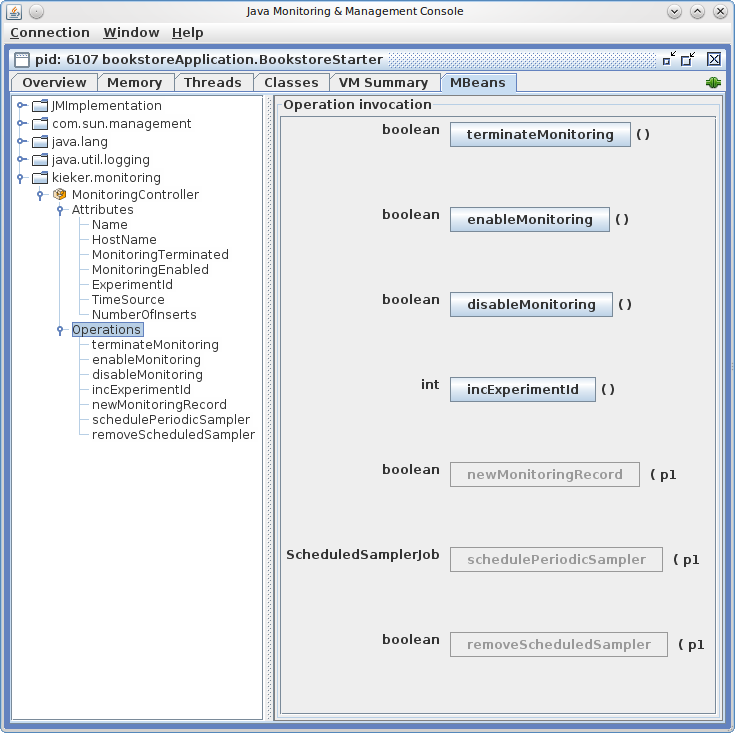
\includegraphics[width=0.485\textwidth]{images/jmxbean-monitoringcontroller-operations.png}
}
\caption{Screenshots of the \class{jconsole} JMX client accessing the \class{MonitoringController}'s %
attributes and operations via the MBean interface. %
}
\label{fig:monitoringController:MBean:jconsole}
\end{figure}

The \class{MonitoringController}'s %
interface methods (see Figure~\ref{fig:monitoringController:classdiagram}) can be accessed %
as a JMX MBean. For example, this allows to control the monitoring state using %
the methods described in the previous Section~\ref{sec:componentsMonitoring:monitoringController:controState}. %
As a JMX-compliant graphical client that is included in the JDK, \class{jconsole} %
is probably the easiest way to get started. Figure~\ref{fig:monitoringController:MBean:jconsole} %
shows two screenshots of the MBean access using \class{jconsole}.

In order to enable JMX MBean access to the \class{MonitoringController}, the value of the %
configuration property \textit{kieker.monitoring.MBean} must be set to \textit{true} (listing below). %
The \file{\monitoringPropertiesFile} includes additional JMX-related configuration properties. \\

\setPropertiesListing
\begin{lstlisting}
 # Whether the MonitoringController will be available as an MBean.
kieker.monitoring.MBean=true
\end{lstlisting}

\subsection{Adaptive Monitoring}

The \class{MonitoringController} provides an API to activate and deactivate %
probes at runtime. By passing a method signature---e.g., %
\texttt{"public void Bookstore.getBook()"}---to the method %
\method{isProbeActivated}, probes can check whether or not monitoring for the %
method with the given signature is active. %
Monitoring can be (de)activated for single signature \textit{patterns}---e.g., %
\texttt{"public void Bookstore.*(..)"}--- via the methods %
\method{activateProbe} and \method{deactivateProbe}. The current list of %
(de)activated patterns can be obtained via the method \method{getProbePatternList}. %
The entire list can be replaced using the method \method{setProbePatternList}. %
Alternatively, a file with include and exclude patterns can be used. This file %
can be polled in regular intervals. %
A default configuration file, including a description of the pattern syntax, is provided %
by the file \file{kieker.monitoring.adaptive\-Monitoring.conf} in the %
\dir{META-INF/} directory of the binary release. %

By default, \Kieker{}'s adaptive monitoring feature is deactivated. It can be %
enabled by setting the value of the configuration property %
\lstinline{kieker.monitoring.adaptiveMonitoring.enabled} %
in the \file{\monitoringPropertiesFile} file to \textit{true}. The %
kieker.monitoring.properties includes additional properties to configure the %
adaptive monitoring, e.g., the location of the afore-mentioned file with %
include/exclude patterns and the polling interval for this file. 

\section{\KiekerMonitoringPart{} Configuration}\label{sec:monitoring:configuration}

\KiekerMonitoringPart{} instances can be configured by properties files, %
\class{Configuration} objects, and by passing property values as %
JVM arguments. If no configuration is specified, a default %
configuration is being used. %
Appendix~\ref{sec:appdx:monitoringproperties} lists this default %
configuration with a documentation of all available properties. %
The default configuration properties file, which %
can be used as a template for custom configurations, is provided by the file %
\file{\monitoringPropertiesFile} in the directory \dir{\KiekerDir/META-INF/} of %
the binary release (see Section~\ref{sec:example:downloadInstall}). %


\subsection*{Configurations for Singleton Instances}

In order to use a custom configuration file, its location needs to be passed to %
the JVM using the parameter \textit{kieker.monitoring.configuration} as follows:

\setBashListing
\begin{lstlisting}[caption=,label=lst:monitoringPropertiesPassedToJVM]
#\lstshellprompt# java  #\textbf{-Dkieker.monitoring.configuration=}#<ANY-DIR>/my.kieker.monitoring.properties #[\ldots]#
\end{lstlisting}

\noindent Alternatively, a file named \file{kieker.monitoring.properties} %
can be placed in a directory called \dir{META-INF/} located in the classpath. %
The available configuration properties can also be passed as JVM %
arguments, e.g., \lstinline{-Dkieker.monitoring.enabled=true}. %

\subsection*{Configurations for Non-Singleton Instances}

The class \class{Configuration} provides factory methods to create %
\class{Configuration} objects according to the default configuration %
or loaded from a specified properties file: \method{createDefaultConfiguration}, %
\method{createConfigurationFromFile}, and \method{createSingletonConfiguration}. %
Note, that JVM parameters are only evaluated when using the factory method %
\method{createSingletonConfiguration}. %
The returned \class{Configuration} objects can be adjusted by setting %
single property values using the method \method{setProperty}. %

\section{Monitoring Records}\label{sec:componentsMonitoring:monitoringRecords}

Monitoring records are objects that contain the monitoring data, as mentioned %
in the previous chapters. Typically, an instance of a monitoring record is %
constructed in a monitoring probe (Section~\ref{sec:monitoring:probe}), %
passed to the monitoring controller (Section~\ref{sec:componentsMonitoring:monitoringController}), %
serialized and deserialized by a monitoring %
writer (Section~\ref{sec:monitoring-log-writers}) and a
monitoring reader, and provided to analysis filters (Section~\ref{sec:analysis:controller}). %
Figure~\ref{fig:KiekerCommunicationDiagram} illustrates this life cycle of a monitoring %
record. %

In Chapter~\ref{chap:example}, we've already introduced and used the monitoring %
record type \class{OperationExecutionRecord}. \Kieker{} allows to use custom %
monitoring record types. Corresponding classes must implement the %
interface \class{IMonitoringRecord} shown in Figure~\ref{sec:monitoringrecord:interfacesAndImplementingClasses}. %
The methods \method{initFromArray}, \method{toArray}, \method{getValueTypes} %
are used for serialization and deserialization of the monitoring data contained %
in the record. Alternatively---in order to support the definition of immutable record types---the %
marker interface \class{IMonitoringRecord.Factory} needs to be implemented, requiring the %
implementation of (i)~the \method{toArray} method (as before), (ii)~a %
constructor accepting a values array, and (iii)~a public static \method{TYPES} %
field. The method \method{setLoggingTimestamp} is used by the monitoring controller to %
store the date and time when a record is received by the controller. %
The method \method{getLoggingTimestamp} can be used during analysis to retrieve %
this value. \KiekerMonitoringPart{} provides the abstract class %
\class{AbstractMonitoringRecord} (Figure~\ref{sec:monitoringrecord:interfacesAndImplementingClasses}) %
which already implements the methods to maintain the logging timestamp.

\begin{figure}[ht]\centering
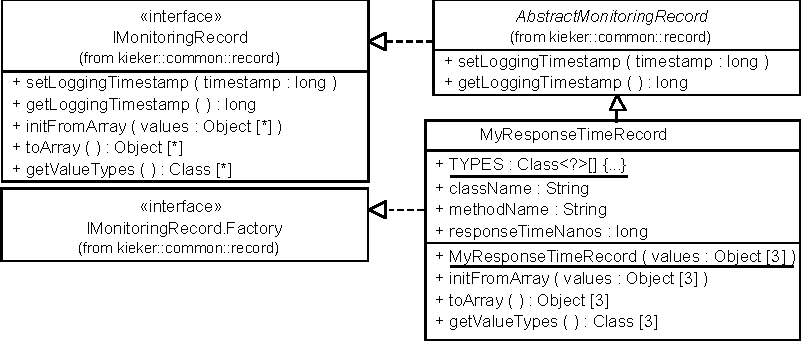
\includegraphics[scale=0.75]{images/kieker_MyRTRecord-modified}
\caption{Class diagram with the \class{IMonitoringRecord} and \class{IMonitoringRecord.Factory} interfaces, the abstract %
class \class{AbstractMonitoringRecord}, and a custom monitoring record type %
\class{MyResponseTimeRecord}}
\label{sec:monitoringrecord:interfacesAndImplementingClasses}
\end{figure}

% \pagebreak

\noindent In order to use the abstract class for implementing your own monitoring record type, you need to:

\begin{enumerate}
\item Create a class that extends \class{AbstractMonitoringRecord}
\item  and
\begin{enumerate}
\item Override the methods \method{initFromArray}, \method{toArray}, \method{getValueTypes}
\item For immutable record types: implement \class{IMonitoringRecord.Factory}, a constructor %
with a single \class{Class<?>[]} argument, and a public static \method{TYPES} field. %
In this case, \method{initFromArray} (which is not called by the framework then) should %
throw an \class{UnsupportedOperationException}.
\end{enumerate}
\end{enumerate}

\noindent The class \class{MyResponseTimeRecord}, shown in the class diagram in %
Figure~\ref{sec:monitoringrecord:interfacesAndImplementingClasses} and in %
Listing~\ref{listing:MyRecord}, is an example of a custom monitoring record type %
that can be used to monitor response times of method executions. %
Implementing \class{IMonitoringRecord.Factory}, \class{MyResponseTimeRecord} is %
an immutable type, i.e., it includes only final fields. %

\pagebreak 

\ % pushing the method initFromArray in the listing to the following page

\setJavaCodeListing
\lstinputlisting[caption=MyResponseTimeRecord.java, label=listing:MyRecord,firstline=22,firstnumber=22]{\customComponentsBookstoreApplicationDir/src/kieker/examples/userguide/ch3and4bookstore/MyResponseTimeRecord.java}

% \pagebreak

\section{Monitoring Probes}\label{sec:monitoring:probe}

The probes are responsible for collecting the monitoring data and passing it %
to the monitoring controller. %
In Chapter~\ref{sec:example:monitoring}, we have already demonstrated how to %
manually instrument a Java application. Listing~\ref{listing:cuttingBookstore} %
shows a similar manual monitoring probe which uses the monitoring record type %
\class{MyResponseTimeRecord} defined in the previous Section~\ref{sec:componentsMonitoring:monitoringRecords}.

% Make sure that this listing will be modified, once the sourcecode changes!!!
% It must show the whole monitoring of the bookstorecall, from getting the first time to persisting of the record!!
\lstinputlisting[firstline=32, lastline=39, firstnumber=32, caption=Excerpt from Bookstore.java, label=listing:cuttingBookstore]{\customComponentsBookstoreApplicationDir/src/kieker/examples/userguide/ch3and4bookstore/Bookstore.java}

\noindent In order to avoid multiple calls to the \method{getInstance} method of the %
\class{MonitoringController} class, singleton instances should be stored %
in a final static variable, as shown in Listing~\ref{listing:cuttingBookstore:finalStaticController}.

\lstinputlisting[firstline=24, lastline=25, firstnumber=24, caption=Singleton instance of the monitoring controller stored in a final static variable (excerpt from Bookstore.java), label=listing:cuttingBookstore:finalStaticController]{\customComponentsBookstoreApplicationDir/src/kieker/examples/userguide/ch3and4bookstore/Bookstore.java}

\noindent When manually instrumenting an application, the monitoring probe is implemented %
by mixing monitoring logic with business logic, which is often not desired since %
the resulting code is hardly maintainable. %
Many middleware technologies, such as Java~EE Servlet~\cite{JavaServletTechnology-WebSite}, %
Spring~\cite{Spring-WebSite}, and %
Apache~CXF~\cite{CXF-WebSite} provide interception/AOP~\cite{Kiczales1997} interfaces %
which are well-suited to implement monitoring probes. AspectJ~\cite{AspectJ-WebSite} allows to %
instrument Java applications without source code modifications. %
Chapter~\ref{chap:aspectJ} describes the \Kieker{} probes based on these technologies allowing to %
monitor trace information in distributed applications.

\section{Monitoring Writers}\label{sec:monitoring-log-writers}

Monitoring writers serialize monitoring records to the monitoring log/stream and  % and persist the recorded informations into files, databases etc. %
must implement the interface \class{IMonitoringWriter}. The monitoring %
controller passes the received records to the writer by calling the method %
\method{newMonitoringRecord}. Writers can use the methods to serialize the %
record contents, as described in Section~\ref{sec:componentsMonitoring:monitoringRecords}.

Figure~\ref{figure:monitoringLogWritersHierarchy} shows the monitoring writers %
already implemented in \KiekerMonitoringPart{}. The available properties for the %
included writers are well-documented in the %
example configuration file (see Appendix~\ref{sec:appdx:monitoringproperties}). %

\enlargethispage{1.2cm}

The writers \class{AsyncFsWriter}, %
\class{SyncFsWriter}, \class{AsyncDbWriter}, and \class{SyncDbWriter} can be used %
to store monitoring records to filesystems and databases respectively. %
The variants with the prefix \class{Async} are implemented using asynchronous %
threads that decouple the I/O operations from the control flow of the %
instrumented application. %
The \class{AsyncFsWriter} is the default writer which has already been used in %
Section~\ref{sec:example:monitoring}. %
Please note that the database writers are currently in a prototype stage and
that they should be used with care. %
The \class{PrintStreamWriter} simply sends the String representation of incoming %
records to the standard output or standard error streams, which can be helpful %
for debugging purposes.

The \class{AsyncJMSWriter} and \class{JMXWriter} write records to a JMS %
(Java Messaging Service~\cite{JMS-WebSite}) queue and JMX (Java Management %
Extensions~\cite{JMX-Website}) queue respectively. The \class{PipeWriter} %
allows to pass records via in-memory record streams (named pipes). %
These writers allow to implement on-the-fly analysis in distributed systems, i.e., analysis while %
continuously receiving new monitoring data from an instrumented application potentially %
running on another machine. A more detailed description of how to use the \class{AsyncJMSWriter} %
can be found in Appendix~\ref{appendix:usingJMS}. %

% This is the diagram with the hierarchy of the writers.
\begin{figure}[H]
\begin{centering}
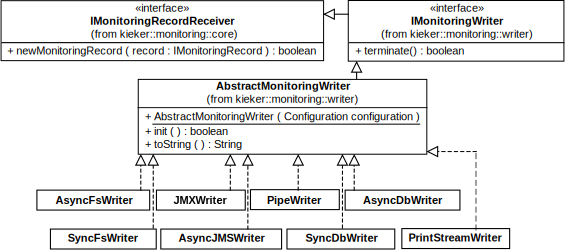
\includegraphics[scale=0.7]{images/kieker_writerimplsuserguide-modified}
\caption{Interface \class{IMonitoringWriter} and  the implementing classes}
\label{figure:monitoringLogWritersHierarchy}
\end{centering}
\end{figure}

\noindent Listing~\ref{listing:MyWriter} %on page~\pageref{listing:MyWriter} 
shows %
a custom writer \class{MyPipeWriter} which uses a named pipe to %
write the given records into a buffer located in the memory. The source code of %
the class \class{MyPipe} is listed in Appendix~\ref{appendix:pipeListings}. %

\enlargethispage{1cm}

\

\setJavaCodeListing
\lstinputlisting[caption=MyPipeWriter.java, label=listing:MyWriter,firstline=23,firstnumber=23]{\customComponentsBookstoreApplicationDir/src/kieker/examples/userguide/ch3and4bookstore/MyPipeWriter.java}

\noindent The monitoring writer to be used is selected by the %
\KiekerMonitoringPart{} configuration property (Section~\ref{chap:componentsMonitoring}) %
\textit{kieker.monitoring.writer}. Writer-specific configuration properties %
can be provided by properties prefixed by the fully-qualified writer classname.  %
Listing~\ref{lst:monitoringwriter:MyWriter} demonstrates how to use the custom %
writer \class{MyPipeWriter} defined above. In this example, the pipe name is %
passed as the property value \textit{pipeName}.

\setPropertiesListing
\lstinputlisting[caption={Configuration of the custom writer \class{MyPipeWriter}},label=lst:monitoringwriter:MyWriter,firstline=5,firstnumber=5,lastline=6]%
{\customComponentsBookstoreApplicationDir/META-INF/kieker.monitoring.properties}

\enlargethispage{1cm}

\noindent As the data structure of this kind of monitoring stream, we created a %
class \class{PipeData} in order to demonstrate the use of the \method{toArray} and %
\method{initFromArray} (in Section~\ref{sec:analysis:reader}) methods. %
A \class{PipeData} object holds a logging timestamp and an \class{Object} array %
containing the serialized record data. %
Appendix~\ref{appendix:pipeListings} includes a source code listing of this class. %
Alternatively, we could have used \class{IMonitoringRecord} as the data structure %
used by the pipe. This is the way, \Kieker{}'s \class{PipeWriter} works. %
